\section{Branch and Bound Approach}
\label{cha:branchandbound}

This chapter is motivated by the fact that branch and bound  search is one of the most widely used tool for solving large scale NP--hard optimization problem. This technique has gained tremendous success in some domain specific areas, such as Boolean satisfiability test (SAT) and mixed integer programming (MIP). In the SAT community, improved versions of the Davis-Putnam-Logemann-Loveland (DPLL) algorithm are able to effectively solve problems with millions of variables and constraints \cite{harmelen}. MIP problems of similar scale can also be solved efficiently using, e.g., CPLEX MIP solver, as shown by \cite{ntaimo}. Despite its success, branch and bound has not been used for 0--1 loss optimization. This chapter, therefore, studies in detail the possible application of this technique in finding the solution of 0--1 loss. Section \ref{sec:bnb.idea} introduces the idea and formulate the 0--1 loss problem in such a way, that it is possible to use branch and bound search. Section \ref{sec:bnb.algorithm} then outlines the basic branch and bound search algorithm for 0--1 loss optimization as an illustration of the branch and bound search concept. Section \ref{sec:bnb.improvement} then proposes several improvements to the basic algorithm in the form of a better initial bound, best-first strategy,  admissible heuristic, and more. Section \ref{sec:bnb.final} discusses the efficiency and effectiveness of all proposed techniques for performance improvement, and proposes the final most effective algorithm for the branch and bound search approach, the performance of which is discussed in \ref{sec:bnb.performance}. A summary is given at the end to conclude all findings of this chapter as well as some directions for future work.



%=================================================
\subsection{Foundation of Branch and Bound Search Approach}
\label{sec:bnb.idea}

This section shows how to formulate the 0--1 loss problem such, that it is possible to apply the branch and bound search strategy. Following from the definition of the 0--1 loss optimization problem given in Chapter \ref{cha:background}, the 0--1 loss function can be written as
$$L(\w) = \sum_{i=1}^N \mathbb{I} [t_i \w^T \xi \leq 0] = \sum_{i=1}^N l_i,$$ 
where $l_i =\mathbb{I} [t_i \w^T \xi \leq 0]$ denotes the individual 0--1 loss of point $\xi$. We have
\[ \begin{split}
l_i = 0 &\Leftrightarrow t_i \w^T \xi > 0 \\
l_i = 1 &\Leftrightarrow t_i \w^T \xi \leq 0. \\
\end{split} \] 
Furthermore, let $\l=(l_1, l_2, \dots, l_N)$ be the loss vector consisting of all individual losses. It can be seen that a specific assignment of the loss vector corresponds to a system of linear inequalities. For example, the loss vector $\l=(0,1,0)$ for a training dataset of $N=3$ points corresponds to
$$
\left\{
     \begin{array}{l}
       t_1 \w^T \x_1 > 0\\
       t_2 \w^T \x_2 \leq 0\\
       t_3 \w^T \x_3 > 0
     \end{array}
\right.
$$
where $t_1, t_2, t_3, \x_1, \x_2, \x_3$ are constants given by the training dataset, so the above is a system of linear inequalities.  

Let $\S_{\l}$ denote the system of linear inequalities induced by the loss vector $\l$.  $\S_{\l}$ can be solved quite efficiently using the well studied linear programming (LP) technique, e.g., by using a LP solver like that by \cite{lpsolve}. There is, however, a subtlety here that needs to be addressed. One can see that if $\w'$ is a solution of $\S_{\l}$, then for any real constant $c > 0$,  $c \w'$ is also a solution. Therefore, if $\S_{\l}$ is consistent, it will have infinitely many solutions. In this case, a LP solver will return a message saying that the solution set is infinite, which is not good because one specific solution is required to determine the decision hyperplane. One trick can be used here is to specify that the bias, $w_0$, must be either $1$ or $-1$, because these are the only two possible values for the bias when $\w$ is scaled by $c=1 / |w_0|$. Here it is assumed that $w_0 \not= 0$, which is reasonable, because otherwise  the decision hyperplane ``must'' go through the origin, which is rare in practice. So, a specific solution of $\S_{\l}$ is obtained by using LP solver to solve for $\{ \S_{\l} \land (w_0=1) \}$ or $\{ \S_{\l} \land (w_0=-1) \}$, whichever has solution. If both these are inconsistent, then $\S_{\l}$ is also inconsistent.

To sum up, a loss vector $\l$ induces a system of linear inequalities, for which a LP solver can either gives a concrete solution $\w'$ if the system is consistent (in this case we call the loss vector \emph{feasible}), or give no solution if the system is inconsistent (in this case we call the loss vector \emph{infeasible}). Thus, the 0--1 loss optimization problem is now equivalent to finding a feasible loss vectors $\l^*$ with minimal sum of its components (which is the sum of  0--1 losses):
$$\l^* = \text{arg min}_{\l : \text{ feasible}} \sum_{i=1}^N l_i.$$
The optimal weight vector, $\w^*$, is then the solution of the system of inequalities induced by $\l^*$ ($\S_{\l^*}$), which can be easily obtained using a LP solver as discussed. 

Clearly, a branch and bound algorithm may be used to find $\l^*$, where in each step we branch on the first unassigned component of the loss vector, $l_i$, for two possible subsets corresponding to $l_i = 0$ or $l_i = 1$. The basic algorithm is detailed in the next section, with more advanced algorithms follow in the section after that.



%=================================================
\subsection{Basic Branch and Bound Algorithm for 0--1 Loss}
\label{sec:bnb.algorithm}

Based on the discussion in the previous section, a possible simple branch and bound algorithm can be constructed as detailed in Algorithm \ref{alg:BnB.Basic} given below. The algorithm takes as input the training dataset $\boldsymbol{X} =  \{ \boldsymbol{x_1, x_2, \dots, x_N } \}$, their training class labels (targets) $\t = \{ t_1, t_2, \dots, t_N \} $, and returns the optimal weight vector $\w^*$.

\begin{figure}
\caption{
Basic Branch and Bound Algorithm for 0--1 Loss Optimization. \\
\text{\hspace{2.2cm}} $Input$: Dataset of training data points $ \boldsymbol{X}$, their labelled class targets $\t$. \\
\text{\hspace{2.2cm}} $Output$: Optimal weight vector $\w^*$ minimizing 0--1 loss.
}
\label{alg:BnB.Basic}
\begin{algorithmic}[1]
\Function{Find-Optimal-01Loss-Solution}{$\X, \t$} \Comment{returns $\w^*$}
\State $loss_{min} \gets +\infty$
\State $\w^* \gets \emptyset$
\State $\l_\emptyset \gets $ loss vector with all components unassigned
\State \Call{Branch-and-Bound}{$\l_\emptyset, 0$}
\State \Return $\w^*$
\Statex
\Procedure{Branch-and-Bound}{$\l, loss$}
   \If {(all components of $\l$ are assigned)}
      \State $\w \gets$ a specific solution of $\S_{\l}$, or $\emptyset$ if inconsistent 
      \If {$\w \not= \emptyset$}
         \State $\w^* = \w$
         \Comment{$\l$ is feasible, update optimal solution}
         \State $loss_{min} \gets loss$
      \EndIf
   \Else
      \State $\l' \gets \l$
      \State Let $i$ be the index of the first unassigned component of $\l$
      \State $l'_i \gets 0$\Comment{Assign 0 to $i-$th component of $\l'$}
      \State \Call{Branch-and-Bound}{$\l', loss$}
      \If {$loss + 1 < loss_{min}$}
         \State $l'_i \gets 1$\Comment{Assign 1 to $i-$th component of $\l'$}
         \State \Call{Branch-and-Bound}{$\l', loss+1$}
      \EndIf
   \EndIf
\EndProcedure
\Statex
\EndFunction
\end{algorithmic}
\end{figure}

The detailed description of each step of the algorithm is as follows. Prior to calling the {\sc Branch-and-Bound} subprocedure, variable $loss_{min}$ is set to $+\infty$ in step 2, $\w^*$ is set to $\emptyset$ in step 3, and all components of the initial loss vector $\l_\emptyset$ is set to be unassigned in step 4. After the execution of the {\sc Branch-and-Bound} procedure in step 5, the value of $\w^*$ -- the optimal solution of 0--1 loss function, is returned in step 6. Steps 7 through 24 belongs to the {\sc Branch-and-Bound} subprocedure. Step 8 checks if all components of $\l$ are assigned (to 0 or 1) then $\l$ is a complete solution. If $\l$ is complete, step 9 assigns $\w$ to a specific solution of $\S_{\l}$ (system of inequalities induced by $\l$) using the trick described in Section \ref{sec:bnb.idea}, or $\w \gets \emptyset$ if $\S_{\l}$ is inconsistent. If $\l$ is feasible, step 11 stores the newly found (better) solution to $\w^*$ and step 12 updates $loss_{min}$ to the new $loss$ value. Note, that $loss$ is always smaller than $loss_{min}$ due to the bounding condition. If, however, $\l$ is not completed, a duplication of $\l$, $\l'$, is created in step 15. Step 16 finds $l_i'$: an unassigned component of $\l'$. Step 17 assigns 0 to $l_i'$, and step 18 branches to this new $\l'$ with the same $loss$, because the total loss value has not been changed. Step 19 is the bounding step as 1 can be assigned to $l_i'$ only if $loss+1$ (the total loss of the current path increased by 1), does not excess the current value of $loss_{min}$. If one additional unit of loss can be assigned, step 20 assigns 1 to the unassigned component, and step 21 branches to the new $\l'$ with the new loss value =  $loss+1$.  


Algorithm \ref{alg:BnB.Basic} is the simplest possible form of branch and bound search for 0--1 loss, and listed rather for illustrational than practical purpose. The algorithm prioritizes branch where $loss$ is not increased, rather than branch where $loss$ is increased (by 1). This is, to some degree, the practice of the best-first strategy and improves the chance to find optimal solution early, hence increases the effectiveness of the bounding step. For example, if the training dataset is separable, the optimal solution will be given immediately in the first time when all components of $\l$ are assigned ($\l$ is completed). For problems with higher optimal loss value, this algorithm is, however, not good enough. For example, it takes over 30 minutes for an implementation of this algorithm in MatLab to solve a problem with size $N=40$ and optimal loss value $loss_{min}=5$ (on a laptop with an average performance). Thus, more sophisticated branching and bounding strategies are required in order to make this approach useful. These strategies will be studied and applied in the next  section.  



%=================================================
\subsection{Techniques for Branch and Bound Improvement}
\label{sec:bnb.improvement}

It was discussed in the previous section, that for the branch and bound (BnB) approach to be practically useful, further improvement is required. Heuristics are well known to be effective mean for this purpose, as detailed in Chapter 3 of \cite{russell}. Thus, this section proposes several heuristics that improve the performance of the basic branch and bound algorithm as detailed in the following three subsections.


%===========================
\subsubsection{Initial Bound Approximation}
\label{sec:bnb.ordering}

The first and simplest technique for performance improvement is to set the initial value of $loss_{min}$ to some initial approximation of the optimal loss value. For example, one can use some fast classifier to approximate the optimal decision hyperplane, then calculate the corresponding 0--1 loss value, and initialize $loss_{min}$ to that value as an initial bound. This technique is rather simple, but quite effective. Basically, all search paths with loss value greater or equal to the value of the initial bound are pruned. For example, if there are 20 points in the training dataset, the number of all possible search paths is $2^{20} \approx 10^6$, if the initial bound is set to 5, the number of search paths to be considered is only ${20 \choose 5} \approx 10^4$, which corresponds to a 100 times reduction in the size of the search space. \footnote{Technically, the reduction is less, because even without an initial approximated bound, the bounding condition at step 19 of Algorithm \ref{alg:BnB.Basic} would still reduce the size of the search tree significantly.} The implementation of this technique is also quite simple and it is included in Algorithm \ref{alg:BnB.BestFirst} at step 5, where the initial bound is set to the loss value induced by the approximated separation hyperplane.    

%===========================
\subsubsection{Best-First Search}
\label{sec:bnb.ordering}

First, let's have a look at an example illustrating the importance of the order, in which components of $\l$ are assigned. For a fictional problem of 40 data points with optimal 0--1 loss = 1, and a fixed assignment order from the first to the last point, if in the optimal solution, the first point is misclassified, then in Algorithm \ref{alg:BnB.Basic}, the loss value of the first component, $l_1$, must be assigned to 1, which would be done only after all combinations where component $l_1$ is $0$ have been checked, which costs $O(2^{39})$, an infeasible number. Clearly, for this example to be feasible,  the resolution is to either have $l_1$ assigned correctly to 1 from the beginning, or change the assignment order such, that $l_1$ is assigned lastly. The strategy discussed in this subsection takes into account both these resolutions.

It was suggested in the previous subsection, that a fast classifier, e.g., logistic regression or linear SVM -- both are $O(N)$, could be used to approximate the optimal decision hyperplane, and then used to approximate the initial bound. It turns out that having an approximated decision hyperplane would also help to determine the assignment order and the assignment value as illustrated in Figure \ref{fig:svm_hyperplane}. Under the assumption that the optimal decision hyperplane is not very far from the approximated hyperplane, clearly, the loss values of points that lies closer to the approximated hyperplane, like point $C$ in the figure, are more likely to be changed comparing to points lying far away, like points $A, B$ in the figure. This fact can be exploited to design a best-first search strategy as follows. The loss values of points farther away from the approximated decision hyperplane are assigned first, and they are assigned to the same loss values as indicated by the approximated decision hyperplane. For example, considering only three points $A, B, C$ in Figure \ref{fig:svm_hyperplane}, the loss value of $B$ would be assigned to 0 first, then the loss value of $A$ assigned to 1, then the loss value of $C$ assigned to 0, then after some branching and bounding, the loss value of $C$ will be changed to 1 in the optimal solution, but the loss values of $A$ and $B$ remain the same.

The above strategy allows to find the optimal solution in a very early stage of the search process. This has twofold benefits. First, it increases the effectiveness of the bounding condition dramatically. Second, if the algorithm reaches time limit and needs to exit, there is a high probability that the current solution is the optimal one, or close to it, and it is guaranteed to be no worse than that of the initial approximation (e.g. given by SVM or some other classifier). As such, it is an $anytime$ algorithm. The algorithm for this best-first search strategy is listed in Algorithm \ref{alg:BnB.BestFirst} with detailed description given in the next paragraph. It is important to mention here, that the distance of point $\xi$ to the decision hyperplane defined by $\w$ is directly proportional to the absolute value of their dot product, $| \xi \cdot \w |$, as detailed in subsection 4.1.1 of \cite{bishop06}, hence the assignment in decreasing order of the distance from given points to the decision hyperplane defined by $\w$ is equivalent to the assignment in decreasing order of the absolute value of their dot product with $\w$. Practical tests on problems of size $N=50$ using the SVM as an initial approximation shows that the time for Algorithm \ref{alg:BnB.BestFirst} to reach the optimal solution in the search tree is on average under 3 seconds. However, it takes much longer  to finish the whole search.

\begin{figure}[here]
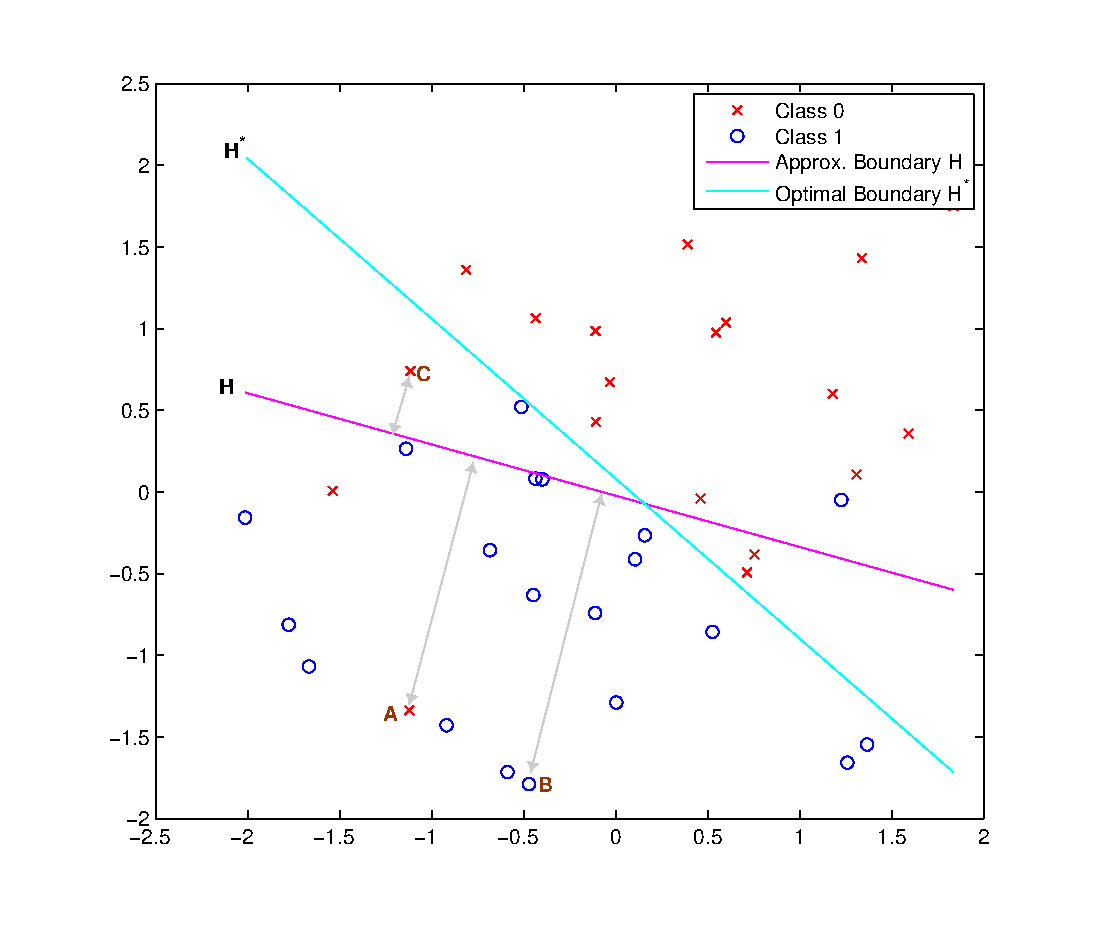
\includegraphics[width=0.50\textwidth]{images/fig31_svmhyperplane.eps}
\caption{
The use of an initial decision hyperplane to direct the loss vector's assignment order and value. 
This plot shows an initial approximated decision hyperplane, $H$, given by the SVM method, with 0--1 loss = 7, the optimal hyperplane, $H^*$, has 0--1 loss = 4. Data point $A$ is misclassified by $H$, hence would have loss value = 1. Data point $B$ is correctly classified, hence would have loss value = 0. Because $A$ and $B$ lie far from $H$, their loss value remains the same when classified by the optimal decision hyperplane $H^*$, which is assumed to not have much deviation from $H$. On the other hand, because point $C$ lies much closer to $H$, its loss value changes when classified by $H^*$. Thus, a good assignment strategy is to assign in order from points farther away to points closer to $H$, and assign the same loss value as classified by $H$ first. 
}
\label{fig:svm_hyperplane}
\end{figure}

The detailed description of each step of Algorithm \ref{alg:BnB.BestFirst} is as follows. Step 2 assigns $\tilde{\w}$ to the weight vector of the approximated separation hyperplane determined by a fast classifier (e.g. by linear SVM). Step 3 assigns $\tilde{\l}$ to be the loss vector induced by $\tilde{\w}$. The initial solution, $\w^*$, is set be the same as $\tilde{\w}$ in step 4, and the initial bound $loss_{min}$ is assigned to corresponding loss determined by $\tilde{\w}$ in step 5. Steps 6-17 are the same as steps 4-15 of Algorithm \ref{alg:BnB.Basic}. Step 18 finds unassigned component $l_i'$ of $\l'$ with greatest value of $|\tilde{\w}^Tx_i|$ (which is analog to greatest distance to hyperplane defined by $\tilde{\w}$). Step 19 assigns a same corresponding loss value of $\tilde{\l}$ to $l_i'$ first, before assigning the opposite value in step 23. Steps 20 and 24 are the bounding conditions to make sure $loss$ is always less than $loss_{min}$. Steps 21 and 25 are branches to the new $\l'$ with the corresponding new loss value.
 
\begin{figure}
\caption{
BnB with Best-First Search for 0--1 Loss Optimization. \\
\text{\hspace{2.2cm}} $Input$: Dataset of training data points $ \boldsymbol{X}$, their labelled targets $\t$. \\
\text{\hspace{2.2cm}} $Output$: Optimal weight vector $\w^*$ minimizing 0--1 loss.
}
\label{alg:BnB.BestFirst}
\begin{algorithmic}[1]
\Function{Find-Optimal-01Loss-Solution}{$\X, \t$}
\State $\tilde{\w} \gets $ approximated weight vector given by a fast classifier
\State $\tilde{\l} \gets $ loss vector implied by $\tilde{\w}$
\State $\w^* \gets \tilde{\w}$
\State $loss_{min} \gets \sum_{i=1}^N \tilde{l}_i$ \Comment{Set initial bound to $L(\tilde{\w})$}
\State $\l_\emptyset \gets $ loss vector with all components unassigned
\State \Call{Branch-and-Bound}{$\l_\emptyset, 0$}
\State \Return $\w^*$
\Statex
\Procedure{Branch-and-Bound}{$\l, loss$}
   \If {(all components of $\l$ are assigned)}
      \State $\w \gets$ a specific solution of $\S_{\l}$, or $\emptyset$ if inconsistent 
      \If {$\w \not= \emptyset$} 
         \State $\w^* = \w$ \Comment{$\l$ is feasible, update optimal solution}
         \State $loss_{min} \gets loss$
      \EndIf
   \Else
      \State $\l' \gets \l$
      \State Find unassigned component $l_i'$ of $\l'$ with greatest value of $|\tilde{\w}^Tx_i|$
      \State $l'_i \gets \tilde{l}_i$\Comment{Assign same loss value as of $\tilde{\l}$ first}
      \If {$loss + l'_i < loss_{min}$}
         \State \Call{Branch-and-Bound}{$\l', loss+l'_i$}
      \EndIf
      \State $l'_i \gets 1 - \tilde{l}_i$\Comment{Then try the opposite loss value}
      \If {$loss + l'_i < loss_{min}$}
         \State \Call{Branch-and-Bound}{$\l', loss+l'_i$}
      \EndIf
   \EndIf
\EndProcedure
\Statex
\EndFunction
\end{algorithmic}
\end{figure}


%===========================
\subsubsection{Loss Propagation}
\label{sec:bnb.heuristic}

This subsection studies the idea of using the convex hull created by data points of a same class to develop a heuristic, which we term \emph{loss propagation}, to improve performance of branch and bound search for 0--1 loss. As shall be seen, loss propagation turns out to be quite powerful as it legitimately enforces some unassigned components of the loss vector to have a specific value, which significantly reduce the search tree and automatically ensures feasibility of the loss vector. 

\begin{figure}[here]
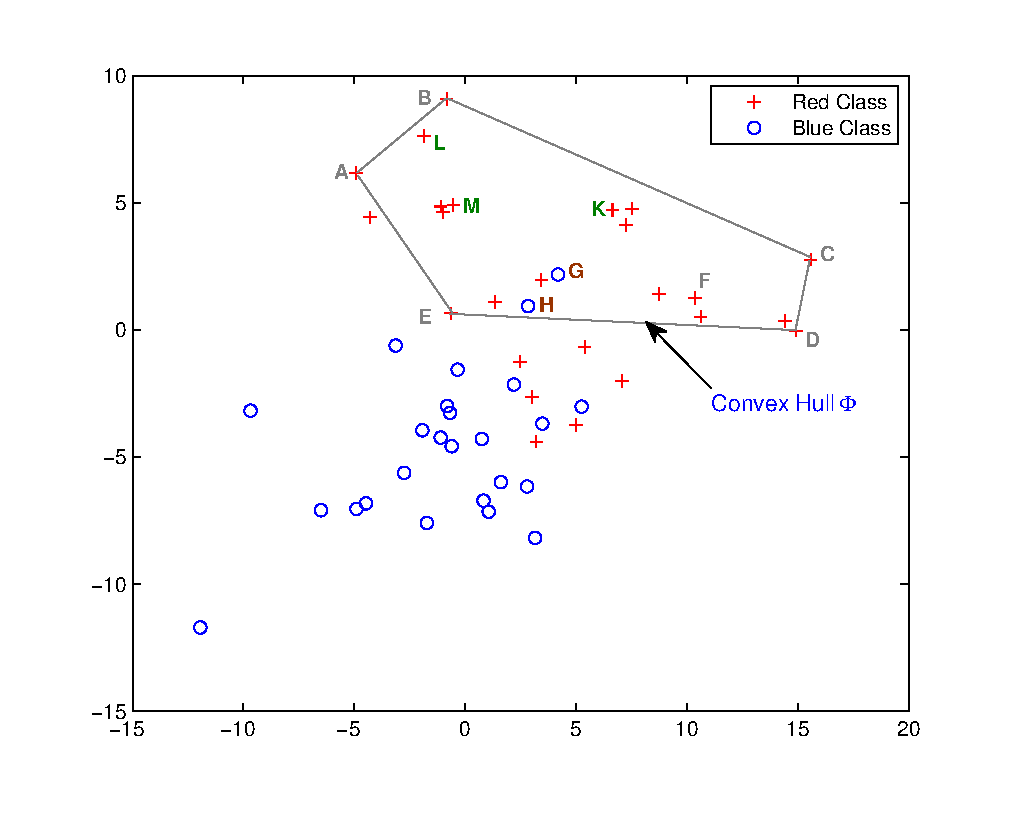
\includegraphics[width=0.50\textwidth]{images/fig32_convexhull.eps}
\caption{
This plot shows that the convex hull created by points, whose loss value has already been assigned, can provide an admissible heuristic and additional pruning.
In this plot, it is assumed, that in the current search path, points $A, B, \dots F$ have loss value assigned to 0, which implies that they are (correctly classified) in the red class, all other points are unassigned. The convex hull $\Phi$ created by points $A$ through $F$ is a convex polygon in this 2D example, and every point inside it must be assigned to the red class in order for the assignment of the loss vector to be feasible. Thus, for example, point $G, H$ must have loss value = 1 (to be misclassified as red class), implying an admissible heuristic value = 2, points $K, M, L$ and all other red points inside $\Phi$ must have loss value = 0 (correctly classified as in red class), hence they require no further branching.
}
\label{fig:convexhull}
\end{figure} 


In Figure \ref{fig:convexhull}, for simplicity it is assumed, that the loss values of data points would be assigned in alphabetical order, i.e., $A, B, \dots, L, \dots $, and in the current search path, loss values of points $A$ through $F$ have been assigned to 0, and loss values of all other points are unassigned. Clearly, points $A$ through $F$ are correctly classified (because their loss is 0), hence they all belong to their true class -- the red class. The convex hull, $\Phi$, of points $A$ through $F$, in this 2--D example, is a convex polygon drawn in grey in the figure. Now, let's consider point $G$, which lies inside the convex polygon $\Phi$. If its loss value is assigned to 0, meaning it is correctly classified as in the blue class, then the set of inequalities induced by the current path is infeasible, because there is no possible decision hyperplane that can separate point $G$ from points $A$ through $F$. Therefore, point $G$ must be misclassified with loss value = 1. Similarly, point $H$ must also have loss value = 1. On the other hand, if point $K$ is misclassified to the blue class, then, again, there's no possible decision hyperplane that can separate it from points $A$ through $F$. Therefore, point $K$ must belong to the red class, and so have loss value = 0. The conclusion is that all points inside the convex hull created by points of a given class must be assigned to that class in order for the assignment to be feasible. Specifically, in Figure \ref{fig:convexhull}, the loss value of all red points inside $\Phi$, such as $K,M,L$, must be 0, the loss value of all blue points, such as $G, H$ must be 1. So we have an admissible heuristic of loss = 2, and forced the loss value of 15 points inside $\Phi$ to be assigned without branching, which is a significant reduction in size of the search tree. 

Another observation is that if, for example, in Figure \ref{fig:convexhull}, in the current search path, points $A$ through $F$ are assigned to the red class, and point $H$ with some (any) other points outside of $\Phi$ are assigned to the blue class, then we can decide that the current loss vector is infeasible, because the two convex hulls created by points of the same class intersect with each other, hence there is no possible decision hyperplane that can separate these two classes. Therefore, in order for the loss vector to be always feasible, we can not assign the loss value of one point, if such assignment makes the two convex hull corresponding to each class intersect with each other. 

The remaining problem to be addressed is how to test if a point $\boldsymbol{p} \in \R^D$ is an interior point of the convex hull created by some other points $\boldsymbol{p_1, p_2, \dots, p_k} \in \R^D$. If points are in $\R^2$, this can be done efficiently in $O(n \log n)$ time, e.g., by determining edges of the convex hull as detailed in Section 33.3 of \cite{cormen}, and then test if the given point is in the correct side of each edge. However, it is not known if any efficient algorithm to determine edges of convex hull in $\R^D$ exists. Thus, we have to approach this problem from another direction using the Barycentric coordinate system, which says point $\boldsymbol{p}$ is an interior point of the convex hull created by points $\boldsymbol{p_1, p_2, \dots, p_k}$ if the homogeneous barycentric coordinates of $\boldsymbol{p}$ with respect to $\boldsymbol{p_1, p_2, \dots, p_k}$ is all non-negative. This is equivalent to solving the following linear programming problem \footnote{This solution was suggested to me by Stephen Gould, CECS, Australian National University.}: find $\boldsymbol{u}$ such that 
$$
u_i \geq 0 \text{ for } i = 1,2, \dots, k \quad \quad \land \quad \quad
\sum_{i=1}^k u_i = 1 \quad \quad \land \quad \quad
\sum_{i=1}^k u_i \boldsymbol{p_i} = \boldsymbol{p}. 
$$
If such $\boldsymbol{u}$ exists, then point $\boldsymbol{p}$ lies in the convex hull of points $\boldsymbol{p_1, p_2, \dots, p_k}$, otherwise it does not. 

To sum up, the above analysis of the convex hull created by the loss assignment identified three possible improvements for the branch and bound search of 0--1 loss. 
\begin{enumerate}
\setlength{\itemsep}{0pt}
\setlength{\parskip}{0pt}
\item All points inside the convex hull of assigned points of one class must be forced to that class. 
\item The sum of forced and assigned components of the loss vector is a lower bound. 
\item If the convex hull of assigned points of one class intersects with that of other class, the current loss vector is infeasible, because no hyperplane can separate the two intersecting convex hulls. Thus, loss value assignment to any point must not make these two convex hulls intersect. 
\end{enumerate}
All these points are accounted in Algorithm \ref{alg:BnB.Heuristics}, where the high level concept should be apparent. A step by step explanation are being provided next for the purpose of an implementation (if needed).
 
\begin{figure}
\caption{BnB with Loss Propagation for 0--1 Loss Optimization}\label{alg:BnB.Heuristics}
\begin{algorithmic}[1]
\Function{Find-Optimal-01Loss-Solution}{$\X, \t$} \Return {$\w^*$}
\State $loss_{min} \gets +\infty$
\State $\w^* \gets \emptyset$
\State $\l_\emptyset \gets $ loss vector with all components unassigned
\State \Call{Branch-and-Bound}{$\l_\emptyset$}
\State \Return $\w^*$
\Statex
\Procedure{Branch-and-Bound}{$\l$}
   \If {(all components of $\l$ are assigned)}
         \State $\w^* \gets$ a specific solution of $\S_{\l}$
         \State $loss_{min} \gets sum(\l)$
   \Else
      \State Let $i$ be the index of the first unassigned component of $\l$
      \State $\l' \gets$ \Call{Propagate-Loss}{$\l, i, 0$}\Comment{branch $l_i=0$}
      \If {$sum(\l') < loss_{min}$}
         \State \Call{Branch-and-Bound}{$\l'$}
      \EndIf
      \State $\l' \gets$ \Call{Propagate-Loss}{$\l, i, 1$}\Comment{branch $l_i=1$}
      \If {$sum(\l') < loss_{min}$}
         \State \Call{Branch-and-Bound}{$\l'$}
      \EndIf
   \EndIf
\EndProcedure
\Statex
\Function{Propagate-Loss}{$\l, i, lossValue$} \Return {new loss vector $\l'$}
   \State $\l' \gets \l$
   \State $l_i' \gets lossValue$   
   \State $\t' \gets $ targets prediction vector implied by $\l'$ 
   \State Let $\Phi =$ convex hull created by $\{ \boldsymbol{x_k} \; | \; t_k'=t_i' \}$ 
   \If {$\exists \boldsymbol{x_j} \in \Phi$ such that $l_j$ is assigned AND $t_j' = -t_j'$}
      \State $l_i' \gets +\infty$ \Comment{convex hulls intersect $\rightarrow$  infeasible}
   \Else
   \For{p:=1 \text{ {\bf to} } N}
      \If{$\boldsymbol{x_p} \in \Phi$ AND $l_p$ unassigned}
         \State $t_p' \gets t_i'$ \Comment{propagate loss to unassigned points inside $\Phi$}
         \State $l_p' \gets \mathbb{I} [t_p' \not= t_p]$
      \EndIf
   \EndFor
   \EndIf  
   \State \Return $\l'$
\EndFunction
\Statex
\EndFunction
\end{algorithmic}
\end{figure}

The detailed description of Algorithm \ref{alg:BnB.Heuristics} is as follows. Steps 1 through 8 are the same as that in the basic algorithm. In contrast to the basic algorithm, however, steps 9 and 10 update the value of $\w^*$ and $loss_{min}$ to the values of the better solution, $\l$, directly without checking for its feasibility. This is possible, because the loss propagation procedure automatically prune all infeasible solutions as will be seen later. Note that $\w^*$ is obtained by solving $\S_{\l}$ (system of inequalities induced by $\l$) using the trick described in Section \ref{sec:bnb.idea}. Step 12 finds the index $i$ of an unassigned component of $\l$. Step 13 calls the {\sc Propagate-Loss} function, which basically returns an admissible heuristic loss vector $\l'$, with the loss value of the $i-$th component assigned to 0, if such assignment is feasible, or $+\infty$ if it is infeasible, and the loss value of all other components updated correspondingly to the aforementioned loss propagation strategy. The value $+\infty$ is assigned to make sure that the infeasible solution is pruned by the bounding condition in step 14. This step also prunes solutions with higher heuristic 0--1 loss than 0--1 loss of the current best solution (hence ensures that the solution found in step 9 is always better than the current best one). Step 15 is just the branching step to the new loss vector $\l'$, which is the result of the loss propagation process corresponding to the assignment of the loss value 0 to the $i-$th component of the current loss vector $\l$. Steps 17 -- 20 are analogous to steps 13 -- 16, except that here the loss value 1 is assigned to the $i-$th component of $\l$ instead of 0. 

Steps 23 through 38 of Algorithm \ref{alg:BnB.Heuristics} belong to the {\sc Propagate-Loss} function, which takes as input the current loss vector $\l$, the index $i$ of an unassigned component of $\l$, and the $lossValue$, either 0 or 1, which will be assigned to the component $i$. This function performs the assignment of loss value of component $i$, propagates this new loss value in accordance with the aforementioned loss propagation process, then returns the result as a new loss vector $\l'$. Specifically, in step 24, $\l'$ is assigned to the current value of $\l$, and $l'_i$,  the $i-$th component of $\l'$, is assigned to the specified value of $lossValue$ in step 25. In step 26, the target prediction vector $\t'$ induced by $\l'$ is determined. Note, that the determination of $\t'$ is easy and is based on the value of $\l'$ and $\t$, which is the true labelled target vector. To be more specific, if $l_i'$ is unassigned then $t_i'$ is undetermined (e.g. set to 0). On the other hand, if $l_i'$ is assigned to 0, the $i-$th component is correctly classified (no loss), implying $t_i' = t_i$, otherwise, $t_i' = -t_i$. Step 27 determines the set of all points $\{ \boldsymbol{x_k} \}$ that are currently assigned to the same class as that of $\xi$ and symbolizes their convex hull as $\Phi$. Step 28 checks if there is any point $\boldsymbol{x_j}$ that is interior point of $\Phi$, and is currently assigned to the class that is opposite to the class of $\xi$. Clearly, if such $\boldsymbol{x_j}$ exists, the assignment $l_i' \gets lossValue$ in step 25 produced an infeasible loss vector $\l'$, because after that assignment, the two convex hulls created by (assigned) points of each class intersect with each other, and this, as has been discussed before, is infeasible because there is no hyperplane that can separate them. So, in this case, step 29 changes the value of $l_i'$ to $+\infty$ to make sure this infeasible solution is pruned by the bounding conditions in step 14 and 18. However, if the solution is feasible, the function continues to step 31 through 36, where the loss propagation is performed. To be more concrete, step 31 and 32 is a for loop and a if condition to check every unassigned point, if it is an interior point of the convex hull $\Phi$, then it must belong to the same class as that of point $\xi$, and step 34 and 35 just update this fact accordingly to the prediction vector $\t'$ and the new loss vector $\l'$. After this loss propagation, all unassigned points that are interior point of $\Phi$ are assigned to the class $t_i'$ of point $\xi$, and their loss value in $\l'$ are updated correspondingly, producing an admissible heuristic 0--1 loss in the form of sum of all assigned components of $\l'$. Finally, step 38 returns the new loss vector $\l'$ after all the feasibility check and loss propagation. 

Note, that the symbol $\Phi$ assigned to represent the convex hull of points $\{ \boldsymbol{x_k} \; | \; t_k'=t_i' \}$ at step 27 only carries a symbolic meaning, as the algorithm to determine vertices (or bounding hyperplanes) of a convex hull of points in $\R^D$ is unknown at this stage. For actual implementation, the set of points $\{ \boldsymbol{x_k} \}$ is maintained instead, and to check if another point $\boldsymbol{x_p}$ is in $\Phi$ is equivalent to solving the linear programming problem $\boldsymbol{Xz=x_p} \land \sum_{i=1}^D z_i = 1 \land \forall i. z_i \geq 0$ as has been discussed earlier in this subsection.

Empirical tests (see Figure \ref{fig:BnBtimes}) shows that for bigger problem ($N>40$), Algorithm \ref{alg:BnB.Heuristics} with the loss propagation heuristic outperforms all other algorithms in this chapter. It is, however, slower for smaller problem. This is expected as with increasing size, the (high) cost to calculate loss propagation starts to pay off. 


%=================================================
\subsection{Evaluation of the Branch and Bound Approach}
\label{sec:bnb.final}

In the following subsections, we propose a final branch and bound algorithm that combines all discussed heuristics and analyze its running time.

%======================
\subsubsection{Combination of Heuristics}

The previous section discussed three strategies to improve the performance of the basic algorithm (Algorithm \ref{alg:BnB.Basic}). Actual implementation and tests (see Figure \ref{fig:BnBtimes}) concludes, that the best algorithm is the one that combines all these strategies. This is an expected result, as the strengths of each strategy would complement each other in a combined algorithm. This combined algorithm is detailed in Algorithm \ref{alg:BnB.Final}.

\begin{figure}[here]
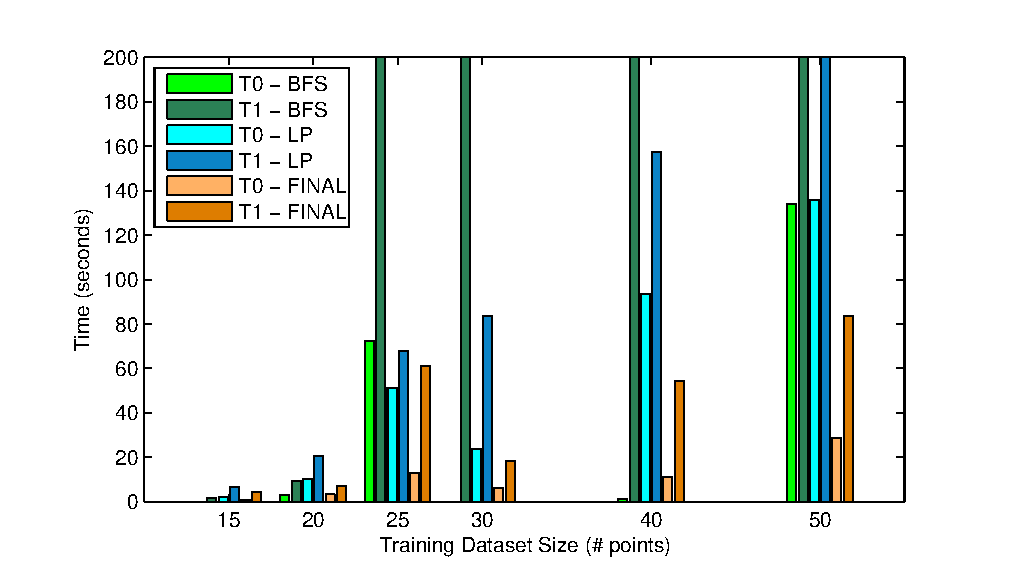
\includegraphics[width=0.50\textwidth]{images/fig33_BnBtimes.eps}
\caption{
This plot compares the time to reach the optimal solution (T0) and the total running time (T1) of best first search algorithm (BFS), loss propagation algorithm (LP), and the final algorithm (FINAL), which combines both BFS and LP. A running time limit of 200 seconds is set for all algorithms. Clearly, BFS reaches the optimal solution early, but takes a long time to finish exploring the whole search space. LP, on the other hand, reaches the optimal solution much slower, and thank to the high cost of  calculating the LP heuristic, it also runs slower than BFS for smaller problems, but it pays off very quickly when $N$ increases, hence outperforms BFS significantly for $N>25$. The combined algorithm, FINAL, has the strengths of both BFS and LP as it reaches the optimal solution early, and  prunes the search space effectively using the loss propagation. Thus, it is the best among these algorithms.}
\label{fig:BnBtimes}
\end{figure} 

The above claim is evidenced by Figure \ref{fig:BnBtimes}, wherein the running times of the best first search (BFS) algorithm, loss propagation (LP) algorithm, and the final algorithm (FINAL) are compared for different problem sizes from $N=15$ to $N=50$ and 0--1 loss value at around 25\% of $N$. A fixed running time limit of 200 seconds is set for all algorithms, so that they will exit and return the best current solution if running time is over 200 seconds. The given result is an average of 10 restarts for each problem's size. The figure shows that for smaller problems, e.g., $N<20$, BFS has advantages over other algorithms, both in the time to reach the optimal solution and in the total running time. This is expected, as the calculation of heuristic in BFS is very fast and simple, and the search is directed toward the optimal solution via the approximation, so the probability of finding optimal solution early is high. LP, on the other hand, reaches the optimal solution much slower, and thank to the high cost of the heuristics calculation, it also runs slower than BFS for smaller problems. But the cost for calculating the loss propagation heuristics pays off very quickly and very well when the size increases. For example, for $N \geq 30$, BFS can not finish the searching process under the given time limit of 200 seconds \footnote{Note, however, that in these cases, the time to reach the optimal solution of BFS is still under 200 seconds, hence the returned result when exiting due to time limit is actually the optimal solution.}, while LP can.  The combined algorithm, FINAL, offers the strengths of both BFS and LP. To be more specific, it reaches the optimal solution very early in search process, and it prunes the search space effectively using the loss propagation heuristics, so that the search is finished under the given time limit even for problem of size 50 and beyond. The running time of the final algorithm clearly shows that it is the best algorithm overall. The pseudocode for the final algorithm is given in Algorithm \ref{alg:BnB.Final}, with description follows in the next paragraph.

\begin{figure}
\caption{
Final BnB Algorithm Combining All Heuristics. \\
\text{\hspace{2.15cm}} $Input$: Dataset of training data points $ \boldsymbol{X}$, their labelled targets $\t$. \\
\text{\hspace{2.15cm}} $Output$: Optimal weight vector $\w^*$ minimizing 0--1 loss.
}
\label{alg:BnB.Final}
\begin{algorithmic}[1]
\Function{Find-Optimal-01Loss-Solution-Final}{$\X, \t$}
\State $\tilde{\w} \gets $ approximated weight vector given by a fast classifier
\State $\tilde{\l} \gets $ loss vector implied by $\tilde{\w}$
\State $\w^* \gets \tilde{\w}$
\State $loss_{min} \gets \sum_{i=1}^N \tilde{l}_i$ \Comment{Set initial bound to $L(\tilde{\w})$}
\State $\l_\emptyset \gets $ loss vector with all components unassigned
\State \Call{Branch-and-Bound}{$\l_\emptyset, 0$}
\State \Return $\w^*$
\Statex
\Procedure{Branch-and-Bound}{$\l, loss$}
   \If {(all components of $\l$ are assigned)}
      \State $\w^* \gets$ a specific solution of $\S_{\l}$ \Comment{update optimal solution}
      \State $loss_{min} \gets loss$
   \Else
      \State Find index $i$ of the unassigned component of $\l$ with greatest $|\tilde{\w}^Tx_i|$
      \State $\l' \gets$ \Call{Propagate-Loss}{$\l, i, \tilde{l}_i$}
      \If {$sum(\l') < loss_{min}$}
         \State \Call{Branch-and-Bound}{$\l'$}
      \EndIf
      \State $\l' \gets$ \Call{Propagate-Loss}{$\l, i, 1 - \tilde{l}_i$}
      \If {$sum(\l') < loss_{min}$}
         \State \Call{Branch-and-Bound}{$\l'$}
      \EndIf
   \EndIf
\EndProcedure
\Statex
\EndFunction
\end{algorithmic}
\end{figure}

In Algorithm \ref{alg:BnB.Final}, steps 2 through 8, which assign variables to their initial values given by an approximation, are the same as step 2 through 8 of the best first search algorithm (Algorithm \ref{alg:BnB.BestFirst}). Steps 10 through 24 that create the body of the {\sc Branch-and-Bound} procedure are identical to steps 8 through 21 of the loss propagation algorithm (Algorithm \ref{alg:BnB.Heuristics}), except for steps 14, 15 and 19, which are explained as follows. Step 14 find the index $i$ of an unassigned component $l_i$ of loss vector $\l$ satisfying the condition, that the distance from the corresponding point $\xi$ to the approximation hyperplane defined by $\tilde{\w}$ is the greatest among all other unassigned points. This distance is directly proportional to $|\tilde{\w}^Tx_i|$ as has been discussed before. Step 15 call the function {\sc Propagate-Loss} to calculate the new loss vector $\l'$, which is the result of loss propagation when the same loss value as predicted by the approximation hyperplane ($\tilde{l}_i$) is assigned to component $l_i$, because this has higher probability of being true (hence must have higher branching priority). Step 19 does the same thing as step 15, however, the opposite loss value to $\tilde{l}_i$ is assigned to $l_i$. Note, that function {\sc Propagate-Loss} was already given in steps 23 through 39 of Algorithm \ref{alg:BnB.Heuristics}, and explained therein. 


%======================
\subsubsection{Running Time Analysis}
\label{sec:bnb.performance}

This section aim to give a rough idea about the complexity and running time of the final branch and bound algorithm as the problem's size increases. Firstly, it should be noted, that the analytical path to determination of the average performance is not easy at all, and the main complication lies in the loss propagation process. It's hard to know how many points are pruned by loss propagation, as this is really problem dependent. One possible approach is to assume a specific family of distribution which generates the data with some parameters $\theta$, and then work out the probability of pruning rate at each step. This, however, is much beyond the scope of this thesis. There is, however, another way to determine the average performance of an algorithm, which is via practical tests, and this is the topic of the next paragraph. The worst case performance, on the other hand, can be easily spotted out as $O(2^N)$, because one can construct an example, which nullify the effect of the loss propagation heuristic. This may look like a big number, but SAT and MIP solvers mentioned earlier in this chapter also have similar worst case performance, yet they work well and have significant importance in practice.     

\begin{table}[h]
\centering
\begin{tabular}{c  c c c c c}
\hline\hline
$N$ & $D$ & 0--1 Loss & T0 & T1 \\
\hline
100 & 3 & 22 & 145 & 1055 \\
200 & 3 & 43 & 710 & 3636 \\
\hline\hline
\end{tabular}
\caption{Results of the initial probing test on two problems. T0 is time to reach the optimal solution. T1 is total running time.} 
\label{tab:inittest}
\end{table}

To probe the performance of the final BnB algorithm (Algorithm \ref{alg:BnB.Final}), an initial test were conducted on two problems with results shown in Table \ref{tab:inittest}. Clearly, the search space for $N=100$ is $\mathcal{S}_1=2^{100} \approx 10^{30}$, and for $N=200$ is $\mathcal{S}_2=2^{200} \approx 10^{60}$, which means the search space has increased by about $10^{30}$ times. On the other hand, the running time has only increased by about 3.5 times, which roughly suggests a polynomial relationship between the running time and the problem's size. 

\begin{figure}[here]
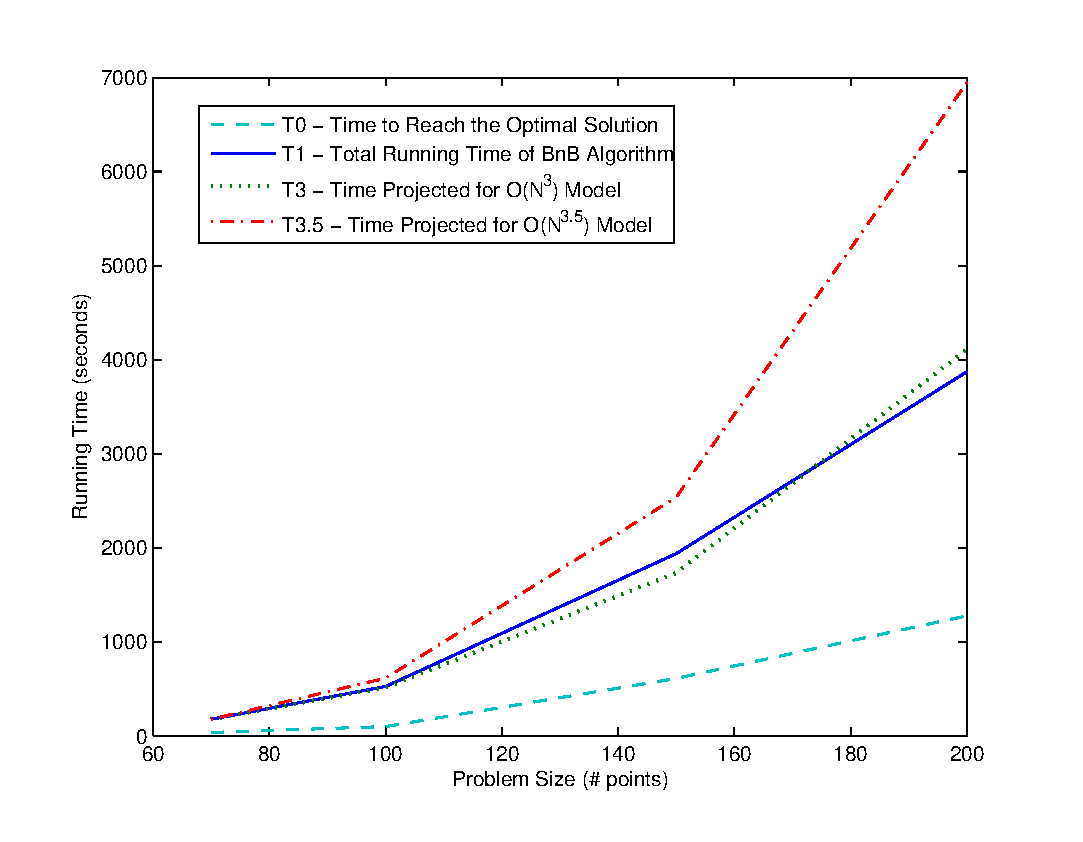
\includegraphics[width=0.50\textwidth]{images/fig34_FinalTimes.eps}
\caption{
This plot shows the time to reach the optimal solution (T0) and the total running times (T1) of the final BnB algorithm with increasing problem's size. Two other times, T3 and T3.5, are projected under assumptions that (a) the underlying algorithm has complexity of $O(N^3)$ and $O(N^{3.5})$ correspondingly, and (b) these times are the same as time T1 at $N=70$. For each problem's size of $N = 70, 100, 150, 200$, ten different problems are generated and tested, each with 0--1 loss $\approx 0.25 N$, and the results shown in the plot are their average values. The plot shows that the running time T1 matches quite closely with T3, and is always upper bounded by T3.5. So for this test, the average running time of the final BnB algorithm seems to be $O(N^3)$.}
\label{fig:FinalTimes}
\end{figure} 

Motivated by the initial test above, a more thorough test has been designed as follows. For each problem's size $N = 70, 100, 150, 200$, ten different problems are generated and tested, each with Loss $\approx 0.25 N$, and the average results over 10 runs are shown in Figures \ref{fig:FinalTimes}. Note, that apart from the time for the algorithm to reach the optimal solution (T0) and the total running time (T1), there are two other times plotted in the figure: T3 and T3.5. These are projected times corresponding to the assumption that the algorithm has complexity $O(N^3)$ or $O(N^{3.5})$ correspondingly. The test result plotted in Figure \ref{fig:FinalTimes} shows that the running time of the final BnB algorithm in this test seems to have $O(N^3)$ average running time. Note that the test for interior point of a convex hull of other points using LP solver is the main bottleneck in the loss propagation calculation, and is well known to be $O(n^3)$, where $n$ is the number of points forming the convex hull (which varies roughly from $1$ to $N/2$ during the search process). Considering this fact, we see that the heuristics implemented in the BnB final algorithms do a decent job in pruning the search space. This test, however, has several flaws. Firstly, the density of points increase with increasing size, so the loss propagation becomes more effective with increasing $N$. Secondly, synthetic testing datasets are continuous under gaussian distribution, while real world data may be discrete and non-gaussian. 


%=================================================
\subsection{Summary}
\label{sec:bnb.summary}

In this chapter, the basic algorithm that uses branch and bound search to find solution of 0--1 loss optimization problem has been designed. Then different strategies to boost the performance have been analyzed and combined into one final best algorithm -- Algorithm \ref{alg:BnB.Final}. While the basic algorithm would give up on problems of size around $N=30$, the final algorithm can solve problems of size $N=200$ and beyond. This number may look small comparing to the power of solvers in other areas like SAT or MIP mentioned at the beginning, but it should be noted, that those solvers were results of over a decade of research and there was a massive amount of investment into each area (circuit verification and operation research), whereas the development of branch and bound algorithm in this chapter is merely for the proof-of-concept purpose. In fact, the final branch and bound algorithm is quite successful in the concept proving role, as it seems to have \emph{average} running time $O(N^3)$ in a given test. Moreover, the algorithm also directs the search to find the optimal solution very early, often in much less time than one third of the total running time, which makes it a good anytime algorithm: the solution returned while having to exit after reaching a time threshold is at least as good as the initial approximation, and there is a good chance that it is the optimal, or near to the optimal solution. The initial approximation can be made by, e.g, logistic regression or linear SVM, both has linear running time. In this case, the returned solution of the final branch and bound algorithm is guaranteed to be better, or at least comparable with the initial approximation.

Algorithms from other approaches that are introduced in subsequent chapters of this thesis are able to work with bigger problems than the current version of the branch and bound algorithm analyzed herein. However, as as shall be discussed in Section \ref{sec:concl.futurework} of the last chapter, there is a real possibility to improve the performance of the branch and bound approach significantly, and if this was made possible, the given final branch and bound algorithm may become one of the best algorithms for the given purpose. This is why branch and bound should have an important place in the discussion of 0--1 loss optimization. More tests to compare different approaches with each other, and with other state-of-the-art methods, as well as tests on real world datasets, are given in Chapter \ref{cha:results}. 
